% ============================================================================
% SECTION 2: INNER WORKINGS
% ============================================================================

\section{Inner Workings}

% ----------------------------------------------------------------------------
% Slide 2.1: Architecture Overview
% ----------------------------------------------------------------------------
\begin{frame}{Architecture Overview}
    \begin{center}
    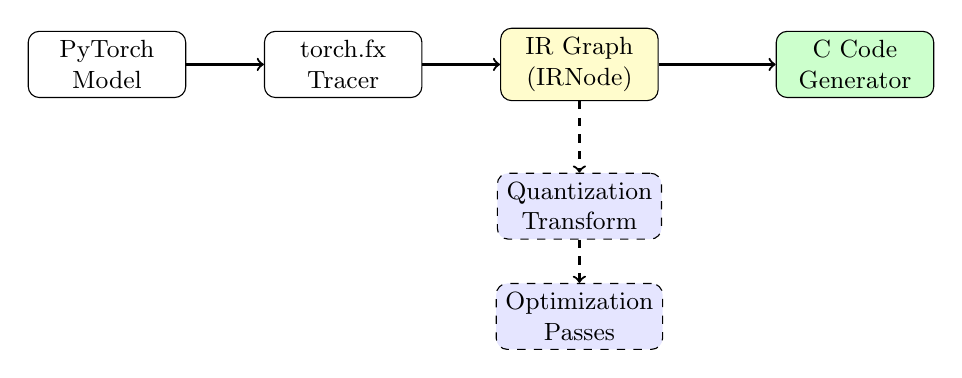
\begin{tikzpicture}[
        box/.style={draw, rounded corners, minimum width=2cm, minimum height=0.8cm, align=center, font=\small},
        optbox/.style={draw, rounded corners, dashed, minimum width=2cm, minimum height=0.8cm, align=center, font=\small, fill=blue!10},
        arrow/.style={->, thick}
    ]
        \node[box] (pytorch) at (0,0) {PyTorch\\Model};
        \node[box] (fx) at (3,0) {torch.fx\\Tracer};
        \node[box, fill=yellow!20] (ir) at (6,0) {IR Graph\\(IRNode)};
        \node[box, fill=green!20] (ccode) at (9.5,0) {C Code\\Generator};
        
        \draw[arrow] (pytorch) -- (fx);
        \draw[arrow] (fx) -- (ir);
        \draw[arrow] (ir) -- (ccode);
        
        \node[optbox] (quant) at (6,-1.8) {Quantization\\Transform};
        \node[optbox] (passes) at (6,-3.2) {Optimization\\Passes};
        
        \draw[arrow, dashed] (ir) -- (quant);
        \draw[arrow, dashed] (quant) -- (passes);
    \end{tikzpicture}
    \end{center}
    
    \vspace{0.5em}
    
    \textbf{Key files:}
    \begin{itemize}
        \item \texttt{frontend/fx\_tracer.py} -- torch.fx tracing
        \item \texttt{lowering/lower.py} -- FX $\rightarrow$ IR conversion
        \item \texttt{ir/graph.py} -- IR graph structure
        \item \texttt{codegen/c\_printer.py} -- C code generation
    \end{itemize}
\end{frame}

% ----------------------------------------------------------------------------
% Slide 2.2: IR Node Structure
% ----------------------------------------------------------------------------
\begin{frame}[fragile]{IR Node Structure}
    \textbf{Base class:} \texttt{src/pytorch\_to\_c/ir/node.py}
    
\begin{lstlisting}[style=pythonstyle]
class IRNode:
    def __init__(self, name, op_type, inputs=None, dtype='float32'):
        self.name = name           # Unique identifier
        self.op_type = op_type     # 'linear', 'conv2d', 'relu', etc.
        self.inputs = inputs or [] # List of input IRNodes
        self.users = []            # Nodes that use this output
        self.dtype = dtype         # 'float32', 'int8', 'int16'
        self.output_shape = None   # Inferred shape
        self.metadata = {}         # Extra info (weights, etc.)
    
    def get_c_dtype(self) -> str:
        """Returns C type: 'float', 'int8_t', 'int16_t'"""
\end{lstlisting}

    \vspace{0.5em}
    \textbf{Graph is doubly-linked:} \texttt{inputs} + \texttt{users} enable traversal in both directions
\end{frame}

% ----------------------------------------------------------------------------
% Slide 2.3: IR Graph Structure
% ----------------------------------------------------------------------------
\begin{frame}[fragile]{IR Graph Structure}
    \textbf{File:} \texttt{src/pytorch\_to\_c/ir/graph.py}
    
    \begin{columns}
    \begin{column}{0.5\textwidth}
\begin{lstlisting}[style=pythonstyle]
class IRGraph:
    def __init__(self):
        self.nodes = []
        self.inputs = []
        self.outputs = []
        self.parameters = {}
    
    def print_graph(self):
        """Pretty-print graph"""
\end{lstlisting}
    \end{column}
    \begin{column}{0.5\textwidth}
        \textbf{Example IR output:}
\begin{lstlisting}[style=diagramstyle]
x [input] dtype=float32
  inputs: []
  users: [fc1]
fc1 [linear] dtype=float32
  inputs: [x]
  users: [relu]
  shape: (1, 8)
\end{lstlisting}
    \end{column}
    \end{columns}
\end{frame}

% ----------------------------------------------------------------------------
% Slide 2.4: Quantization Rule System
% ----------------------------------------------------------------------------
\begin{frame}[fragile]{Quantization Rule System}
    \textbf{Base class:} \texttt{src/pytorch\_to\_c/quantization/rules.py}
    
\begin{lstlisting}[style=pythonstyle]
class QuantRule(ABC):
    def __init__(self, pattern: str, dtype: str):
        self.pattern = re.compile(pattern)  # Regex for layer names
        self.dtype = dtype                   # 'int8' or 'int16'
    
    def matches(self, node: IRNode) -> bool:
        """Check if rule applies to this node"""
        return self.pattern.search(node.name) is not None
    
    @abstractmethod
    def create_quant_node(self, float_node: IRNode) -> QuantIRNode:
        """Create quantized version of the node"""
\end{lstlisting}

    \vspace{0.5em}
    \textbf{Rule matching:} First matching rule wins
\begin{lstlisting}[style=pythonstyle]
RuleMatcher([rule1, rule2, rule3])  # Checked in order
\end{lstlisting}
\end{frame}

% ----------------------------------------------------------------------------
% Slide 2.5: Writing a Custom Rule
% ----------------------------------------------------------------------------
\begin{frame}[fragile]{Writing a Custom Rule}
    \textbf{Example: Static Quantization Rule}
    
\begin{onlyenv}<1>
\begin{lstlisting}[style=pythonstyle]
class StaticQuantRule(QuantRule):
    def __init__(self, pattern, dtype, 
                 input_scale, weight_scale, output_scale, ...):
        super().__init__(pattern, dtype)
        self.input_scale = input_scale
        # ... store all scales/offsets
\end{lstlisting}
\end{onlyenv}

\begin{onlyenv}<2>
\begin{lstlisting}[style=pythonstyle]
class StaticQuantRule(QuantRule):
    def __init__(self, pattern, dtype, 
                 input_scale, weight_scale, output_scale, ...):
        super().__init__(pattern, dtype)
        self.input_scale = input_scale
    
    def create_quant_node(self, float_node: IRNode) -> QuantIRNode:
        if float_node.op_type == 'linear':
            return StaticQuantLinearNode(
                name=float_node.name, dtype=self.dtype,
                input_scale=self.input_scale, ...
            )
        elif float_node.op_type == 'conv2d':
            return StaticQuantConv2dNode(...)
\end{lstlisting}
\end{onlyenv}
\end{frame}

% ----------------------------------------------------------------------------
% Slide 2.6: Quantized Node Structure
% ----------------------------------------------------------------------------
\begin{frame}[fragile]{Quantized Node Structure}
    \textbf{Base class:} \texttt{src/pytorch\_to\_c/ir/quant\_node.py}
    
\begin{lstlisting}[style=pythonstyle]
class QuantIRNode(IRNode):
    """Base class for all quantized operations"""
    
    @abstractmethod
    def get_pre_nodes(self) -> List[IRNode]:
        """Nodes to insert BEFORE this op (e.g., QuantizeNode)"""
    
    @abstractmethod
    def get_post_nodes(self) -> List[IRNode]:
        """Nodes to insert AFTER this op (e.g., DequantizeNode)"""
    
    @abstractmethod
    def generate_c_code(self, c_printer) -> str:
        """Generate the C code for this operation"""
\end{lstlisting}

    \vspace{0.5em}
    \textbf{Key insight:} Each QuantIRNode controls its own conversion nodes!
\end{frame}

% ----------------------------------------------------------------------------
% Slide 2.7: StaticQuantLinearNode Implementation
% ----------------------------------------------------------------------------
\begin{frame}[fragile]{StaticQuantLinearNode Implementation}
    \textbf{File:} \texttt{src/pytorch\_to\_c/quantization/ops/quant\_linear.py}
    
\begin{onlyenv}<1>
\begin{lstlisting}[style=pythonstyle]
class StaticQuantLinearNode(QuantIRNode):
    def __init__(self, name, dtype, input_scale, weight_scale, ...):
        super().__init__(name, 'linear', dtype=dtype)
        self.input_scale = input_scale
        self.weight_scale = weight_scale
        self.output_scale = output_scale
\end{lstlisting}
\end{onlyenv}

\begin{onlyenv}<2>
\begin{lstlisting}[style=pythonstyle]
    def get_pre_nodes(self):
        return [QuantizeNode(
            name=f"{self.name}_input_q",
            dtype=self.dtype,
            scale=self.input_scale,
            offset=self.input_offset
        )]
    
    def get_post_nodes(self):
        return [DequantizeNode(
            name=f"{self.name}_output_dq",
            scale=self.output_scale,
            offset=self.output_offset
        )]
\end{lstlisting}
\end{onlyenv}

\begin{onlyenv}<3>
\begin{lstlisting}[style=pythonstyle]
    def generate_c_code(self, c_printer):
        return f"dense_int8({input}, {size}, {weight}, " \
               f"{bias}, {out_size}, {self.input_scale}f, " \
               f"{self.weight_scale}f, 0, {output});"
\end{lstlisting}
\end{onlyenv}
\end{frame}

% ----------------------------------------------------------------------------
% Slide 2.8: QuantizationTransform Pipeline
% ----------------------------------------------------------------------------
\begin{frame}[fragile]{QuantizationTransform Pipeline}
    \textbf{File:} \texttt{src/pytorch\_to\_c/quantization/graph\_transform.py}
    
\begin{lstlisting}[style=pythonstyle]
class QuantizationTransform:
    def __init__(self, rules: List[QuantRule]):
        self.matcher = RuleMatcher(rules)
    
    def apply(self, ir_graph: IRGraph) -> IRGraph:
        # Step 1: Find nodes matching rules
        nodes_to_quantize = self._find_nodes_to_quantize(ir_graph)
        
        # Step 2: Replace float nodes with QuantIRNodes
        self._replace_nodes(ir_graph, nodes_to_quantize)
        
        # Step 3: Insert pre/post nodes (Quantize/Dequantize)
        self._insert_node_controlled_conversions(ir_graph)
        
        # Step 4: Validate output is float32
        self._validate_float_output(ir_graph)
        
        # Step 5: Quantize weights
        self._quantize_weights(ir_graph, nodes_to_quantize)
        
        return ir_graph
\end{lstlisting}
\end{frame}

% ----------------------------------------------------------------------------
% Slide 2.9: Adding a New Quantized Operation
% ----------------------------------------------------------------------------
\begin{frame}[fragile]{Adding a New Quantized Operation}
    \textbf{Steps to add \texttt{QuantizedSoftmax}:}
    
    \begin{enumerate}
        \item<1-> \textbf{Create the node class:}
\begin{onlyenv}<1->
\begin{lstlisting}[style=pythonstyle]
class StaticQuantSoftmaxNode(QuantIRNode):
    def get_pre_nodes(self): ...
    def get_post_nodes(self): ...
    def generate_c_code(self, c_printer): ...
\end{lstlisting}
\end{onlyenv}

        \item<2-> \textbf{Add C implementation:}
\begin{onlyenv}<2->
\begin{lstlisting}[style=cstyle]
void softmax_int8(const int8_t* input, int size, 
                  float scale, int offset, int8_t* output);
\end{lstlisting}
\end{onlyenv}

        \item<3-> \textbf{Update rule to create it}
        \item<3-> \textbf{Export in \texttt{\_\_init\_\_.py}}
    \end{enumerate}
\end{frame}

